\chapter{Discussion}
\label{chap:Discussion}
The discussion chapter will describe some of the choices made through the project and problems that have occurred. The problem and choices will be described and discussed, what happened and what could have been done differently. 

\textbf{Scheduling}



%Worst-case execution time analysis
%Hvordan vi har talt clock cycles og den process. - Tools vi har brugt til WCET?
\textbf{Hardware choices}

%Valg af de forskellige shields, ardunio board, sensor. Godt/dårligt, ændringer.
\textbf{Object detection}


%Er der ting vi kunne have gjort anderledes for at få bedre resultater her ?
\textbf{Delimitations}

For this project we made two delimitations to the project, which can be found in section \ref{sec:Delimitations}. As mentioned, only one object will be thrown at any given time. This is an environmental delimitation, to not consider multiple projectiles at once. \newline
Another delimitation made was that the robot should not drive to coordinate points behind itself within the predefined area, but this is actually possible for the robot to do, also outside the predefined area. A problem we should have realized much earlier is that it is not possible for the robot to catch the object, unless it lands extremely close to the robot’s starting position, because of time spent processing and sending a signal, limitations of the motor. Another delimitations should have been made that the robot should not try to catch the object, but rather drive to the point where the object hit the ground. \newline
Instead the predefined area should not be considered and the robot should have a starting point at (0, 0), as shown in figure \ref{figure:graph} as the red dot. The robot should then be able to move to both the blue crosses(direction of the old predefined area, but not limited to the old predefined area) and the green crosses behind the robot’s starting position. 


\begin{figure}[h]
	\centering
	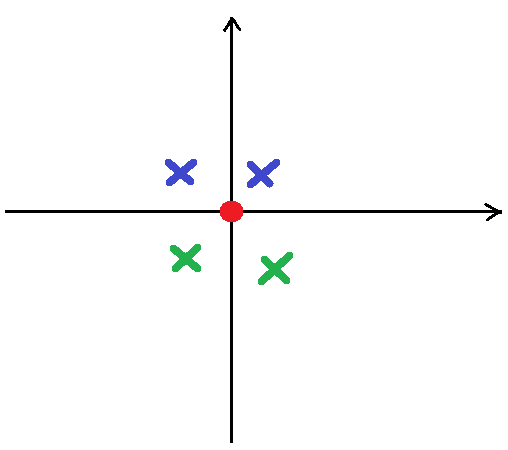
\includegraphics[scale=0.75]{billeder/discussion-graph.png}
	\caption{Graph describing the coordinate set with no predefined area}
	\label{figure:graph}
\end{figure}

\textbf{Process model analysis}

The process model used for this project, which is described in section \ref{Process model}, is a reflection on how our perspective on the processes we usually follow. It is inspired by XP, including pair programming and agile development with incrementally changing requirements. If the solution to our problem would be a safety critical solution, a more test-driven process model would be more suitable. Catching regular trash is not a hard real-time, safety critical task, unless the trash is a threat to human life or mission critical.\newline
The process model itself has worked out rather well since it isn’t restrictive and provides a very large degree of freedom when working with the project compared to a rigid adherence to a well established model such as the waterfall model. \newline
Even though a lot of freedom might be a good thing, it can also be a bad thing for a process model. When working with the process model, it might not have been a good way to structure the work and it has been very experimental at times. \newline
After experimenting with the process model throughout this project it has come to our attention that some changes should be made to the structure of the process model. A more explicit test section should be implemented to test all interdependent components, and ensure that all increments implementations work as intended. This will in turn also increase the coherence between each increment. This test section will also include tests across each increment, to check that no new errors has been introduced to earlier implementation.
%Har vores process model virket? Hvad har virket/hvad har ikke virket? Hvad kan laves om ? Generel reflektion.


%Skulle vi have lavet nogle noget før, om de var nødvendige, om vi skulle have lavet andre, projektets delimitations står som kommentarer herunder:
%The group have made two delimitations for the project. First the group have decided that multiple object thrown should not be considered, so only one object should be thrown at a time. \newline
%It have also been decided that the robot should not drive backwards. The robot starts outside its predefined area and will only drive forward into that. This means that if the robot is already heading towards a point in its predefined area and the Kinect sends a new point, which is behind the robot, it will not be able to drive to the new point given by the Kinect.




%Kunne vi generelt have gjort det til et mere real time problem eller er det overhovedet et godt projekt område til realtids problemer????
%Vi skal huske at referere til det openkinect library vi bruger?????
%Vi ku tage de 10 punkter til safety critical realtids guidelines

